\documentclass[12pt]{article}

\usepackage{stylefile}

\begin{document}

\begin{center}
\noindent\LARGE \textbf{Exclusive disjunction} \\[.5cm]
\large Michael Franke\\[.1cm] 
\large Bob van Tiel
\end{center}

\begin{abstract}
If someone says `Donald ate a pretzel or a donut' you might infer that he did not eat both a pretzel and a donut. This exclusive reading of `or' is often explained as a scalar implicature. We present experimental evidence suggesting that this explanation is on the wrong track.
\end{abstract}

%--------------------------------------------------------
\section{Introduction}
%--------------------------------------------------------
\subsection*{The meaning of `or'}
%--------------------------------------------------------

Introductions to logic usually distinguish two possible interpretations of `or': an inclusive and an exclusive interpretation \citep[e.g.,][]{mccawley1981, copi2005}. The inclusive interpretation corresponds to the meaning of logical disjunction. According to this interpretation, `$A$ or $B$' is true if at least one and possibly both of $A$ and $B$ are true. The exclusive interpretation is more strict in that it precludes the possibility that both $A$ and $B$ are true. In other words, on its exclusive interpretation, `$A$ or $B$' is true if exactly one of $A$ and $B$ is true.

The presence of these two interpretations might lead one to conclude that `or' must be associated with two lexical entries. 
 



According to \emph{lexicalism}, `or' simply has two lexical entries corresponding to the two interpretations. \emph{Univocalists} assume that `or' only has one interpretation, namely the inclusive one, and that the illusion of an exclusive interpretation is due to considerations of world knowledge. Finally, \emph{pragmatists} argue that the primary meaning of `or' is inclusive, but that this inclusive meaning can be strengthened through pragmatic reasoning. 

In the next section, we will discuss these three proposals in more detail.

%--------------------------------------------------------
\subsection*{Inclusive and exclusive `or'}
%--------------------------------------------------------

Although this is usually not spelled out in much detail, many logicians hold that the equivocation between the inclusive and exclusive interpretation of `or' is due to a lexical ambiguity \citep[e.g.,][]{basson1960, baum1996, rescher1964}. Thus, \citet[p.\ 21]{tarski1946} observes that ``[t]he word `or', in everday language, possesses at least two different meanings''.

Perhaps the most important problem with this proposal is that it fails to explain why sometimes only one interpretation is accessible. Consider an utterance of:

\ex.	 Joe does not support Donald or Hillary.

This utterance has only one interpretation, namely that Joe supports neither Donald nor Hillary. This interpretation corresponds to an inclusive reading of `or'. The interpretation corresponding to an exclusive reading, which would imply that Joe either supports both Donald and Hillary or neither of them, is not attested.

More generally, the lexicalist proposal begs the question of how the ambiguity between the inclusive and exclusive interpretation is resolved. Perhaps the most straightforward answer to that question would be to invoke considerations of world knowledge, which brings us to the second proposal.

Perhaps surprisingly, a number of theorists have denied that `or' has more than one interpretation \citep[e.g.,][]{rubin1989, yanal1988}. According to these univocalists, `or' always receives an inclusive interpretation. The appearance of an exclusive interpretation is due to world knowledge considerations. To illustrate, consider an utterance of:

\ex.	Joe voted for Donald or Hillary.

Here, it seems that the speaker's utterance rules out the possibility that Joe voted for both Donald and Hillary. According to univocalism, this inference is not due to an exclusive reading of `or' but rather to an inclusive reading along with the commonsense information that one can only vote once in a democratic election. In this way, then, world knowledge is responsible for seemingly exclusive interpretations of `or'.

The univocalist proposal straightforwardly accounts for the absence of exclusive readings when `or' is embedded under negation:\ world knowledge can only strengthen the inclusive interpretation, and when `or' is embedded under negation the inclusive reading is stronger than the exclusive one.

The pragmatic proposal mirrors the univocalist one in that it assumes that the primary meaning of `or' is inclusive. Instead of attributing exclusive readings to world knowledge inferences, however, pragmaticists argue that they are a variety of scalar implicature \citep[e.g.,][]{horn1972, gazdar1979, sauerland2004, geurts2010}. To illustrate, consider an utterance of:

\ex.	Joe supports Donald or Hillary.

Assuming that the primary meaning of `or' is inclusive, the hearer may reason as follows:\ the speaker could have been more informative by uttering the alternative `Joe supports Donald and Hillary'. Why didn't she? Presumably because she does not believe that the alternative is true. This weak inference, which is compatible with a situation in which the speaker is ignorant about whether or not Joe supports both Donald and Hillary, can be strengthened if the speaker is taken to be competent about whether the alternative is true or false. If so, it follows that, according to the speaker, the alternative is false.

Even though the pragmatic account is usually considered the standard in the current literature, it faces a number of problems. Perhaps the most important of these was first observed by \citet{geurts2006} and dubbed the `speaker expertise paradox' by \citet{zondervan2010}. The speaker expertise paradox arises because utterances with `or' usually imply that the speaker does not know whether the individual disjunctions are true or false. Someone who says \Last, for example, will usually be taken to imply that she does not know whether Joe supports Donald and that she does not know whether Joe supports Hillary.

However, in order to derive the exclusive interpretation as a scalar implicature, it has to be assumed that the speaker knows whether or not Joe supports both Donald and Hillary. In other words, the pragmatic proposal implies that, whenever `$A$ or $B$' is interpreted exclusively, the speaker is ignorant about the truth of $A$ and $B$ but knows that the conjunction `$A$ and $B$' is false. Such an epistemic state is possible but intuitively improbable, which contradicts the observation that exclusive interpretations are far from uncommon.

%--------------------------------------------------------
\subsection*{Testing the three proposals}
%--------------------------------------------------------

In order to decide between the three proposals discussed in the previous section, we tested how the robustness of the exclusive interpretation is influenced by three factors:\ (i) the relevance of the corresponding statement with `and' for the hearer, (ii) the competence of the speaker about the statement with `and', and (iii) the prior probability that the statement with `and' is true. 


%--------------------------------------------------------
\section{Experiment 1}
%--------------------------------------------------------
\subsection*{Design}
%--------------------------------------------------------

Our goal is to find out whether three contextual factors have an influence on the strength of
exclusive disjunction readings: (i) the \emph{relevance} of the truth of the conjunction for
the listener, (ii) the \emph{competence} of the speaker (i.e., whether the speaker is likely to
know if the conjunction is true), and (iii) the \emph{prior probability} of the conjunction, in
terms of common-sense expectations about likely worldly events irrespective of what was
said. To measure these factors and the strength of disjunctive readings, we designed different
contexts (vignettes) that systematically varied along the three relevant factor dimensions.  We
used a slider-rating task to assess participants' intuitive judgement of all four notions of
interest: strength of exclusive inference, relevance, competence and prior probability.

We used a between-subjects design in which each participant only answered one of the four
relevant test questions for a given vignette. This was to prevent cross-contamination of
answers, e.g., asking first about relevance might influence subsequent answers about strength
of disjunctive readings.


\subsection*{Participants}

200 participants were drafted on Amazon's Mechanical Turk and paid 80 US\$
cent.\footnote{Mechanical Turk is a website where workers perform so-called `Human Intelligence
  Tasks' (HITs) for financial compensation. It has been shown that the quality of data gathered
  through Mechanical Turk equals that of laboratory data (e.g., Buhrmester, Kwang \& Gosling
  \citeyear{buhrmester2011}, \citealt{schnoebelen2010, sprouse2011}).} Payment was not
contingent on any of their responses. Only workers with an IP address from the United States
and with a rate of accepted HITs of at least 90\% were eligible for participation.

\subsection*{Materials}

The materials consisted of sixteen vignettes (see Appendix~\ref{sec:mater-exper-1} for a full
list). Each vignette came with a background story and an utterance of a
disjunctive statement by some character. For example:

\begin{quote}
  \emph{Background story} \\
  Danny and Alex reserved a squash court but Alex still has to buy a racket and a pair of
  shoes. Danny is talking to Alex's girlfriend Jill who just went to the sports store with
  him.\\[.2cm]
  \emph{Utterance of disjunction}\\
  Jill says to Danny: `Alex bought a racket or a pair of shoes.'
\end{quote}

\noindent Each vignette was associated with three control statements which were either
certainly true, certainly false, or of uncertain truth value, given the background
story. Moreover, each vignette was also associated with four target statements gauging (i) the
strength of exclusive inference, (ii) the relevance of the truth of the conjunction for the
listener, (iii) the competence of the speaker, and (iv) the prior probability of the
conjunction. The four target statements associated with the example above were:

\begin{quote}
  \emph{Xor}\\
  From what Alex's girlfriend said we may conclude that Alex did not buy both a racket and a
  pair of shoes.\\[.2cm]
  \emph{Relevance} \\ It is important for Danny to know whether Alex bought both a racket and a
  pair of shoes.\\[.2cm]
  \emph{Competence} \\ Alex's girlfriend knows whether he bought both a racket and a pair of shoes. \\[.2cm]
  \emph{Prior} \\ If Alex bought a racket, it is likely that he also bought a pair of shoes. \\
  If Alex bought a pair of shoes, it is likely that he also bought a racket.
\end{quote}

\noindent Statements \emph{Xor}, \emph{Relevance} and \emph{Competence} were single
sentences. Statements \emph{Prior} were pairs of symmetric conditional statements, where each
targeted the intuitive probability that, given one disjunct, the other would be true as
well. We reasoned that this makes for more natural statements and that it may give us more
reliable measures than having subjects rate a single conjunctive
statement. Section~\ref{sec:experiment-2:-prior} picks up this topic and presents a follow-up
experiment using the latter alternative method for measuring prior expectations.

The vignettes were created to ensure sufficient variability across the three dimensions of
interest (i.e., relevance, competence and prior). We classified each vignette according to
whether we felt it to be high or low on each dimension, thus making for eight types of
vignettes. We had two vignettes for each type. For example, we expected the vignette above to
score high on all three dimensions. A full list of the sixteen vignettes, together with our
intuitive type-classification, can be found in Appendix~\ref{sec:mater-exper-1}. \mf{insert
  appendices with materials}

\subsection*{Procedure}

The experiment started with instructions:

\begin{quote}
  In the following, you will be presented with 8 short background stories. Please read them
  very carefully. We ask you to rate 2 or 3 statements for each background story. Please
  indicate, using an adjustable slider, how likely you think a statement is true based on the
  background story.
\end{quote}

\noindent Next, we presented a simple background story which was not used in the main
experiment, followed by three annotated examples to illustrate the use of the slider bar. One
example was clearly true, another clearly false, and the last uncertain.

In the main part of the experiment, every participant saw eight randomly sampled vignettes, one
of each vignette type, in random order. Each vignette was followed first by one random control
statement and then the statement(s) associated with one of the four factors of interest
(relevance, competence, prior or xor). Each participant rated each of the four statement types
exactly twice, but never in direct succession. When the prior statements were presented, only
the background story was provided, but not the disjunctive statement, so as to make sure that
answers are based on expectations about worldly events alone, unmodulated by information based
on pragmatic inferences from utterances. All other question types had the background story and
the disjunctive statement appear on the screen. The two prior statements were presented
individually, one after the other, in random order.

Ratings of statements were elicited by asking ``How likely do you think it is that the
statement is true, given the information in the background story?'' together with a continuous
slider ranging from ``certainly false'' to ``certainly true.'' An example of a trial is given
in Figure~\ref{fig:exampleShot}.

\begin{figure}
  \centering
  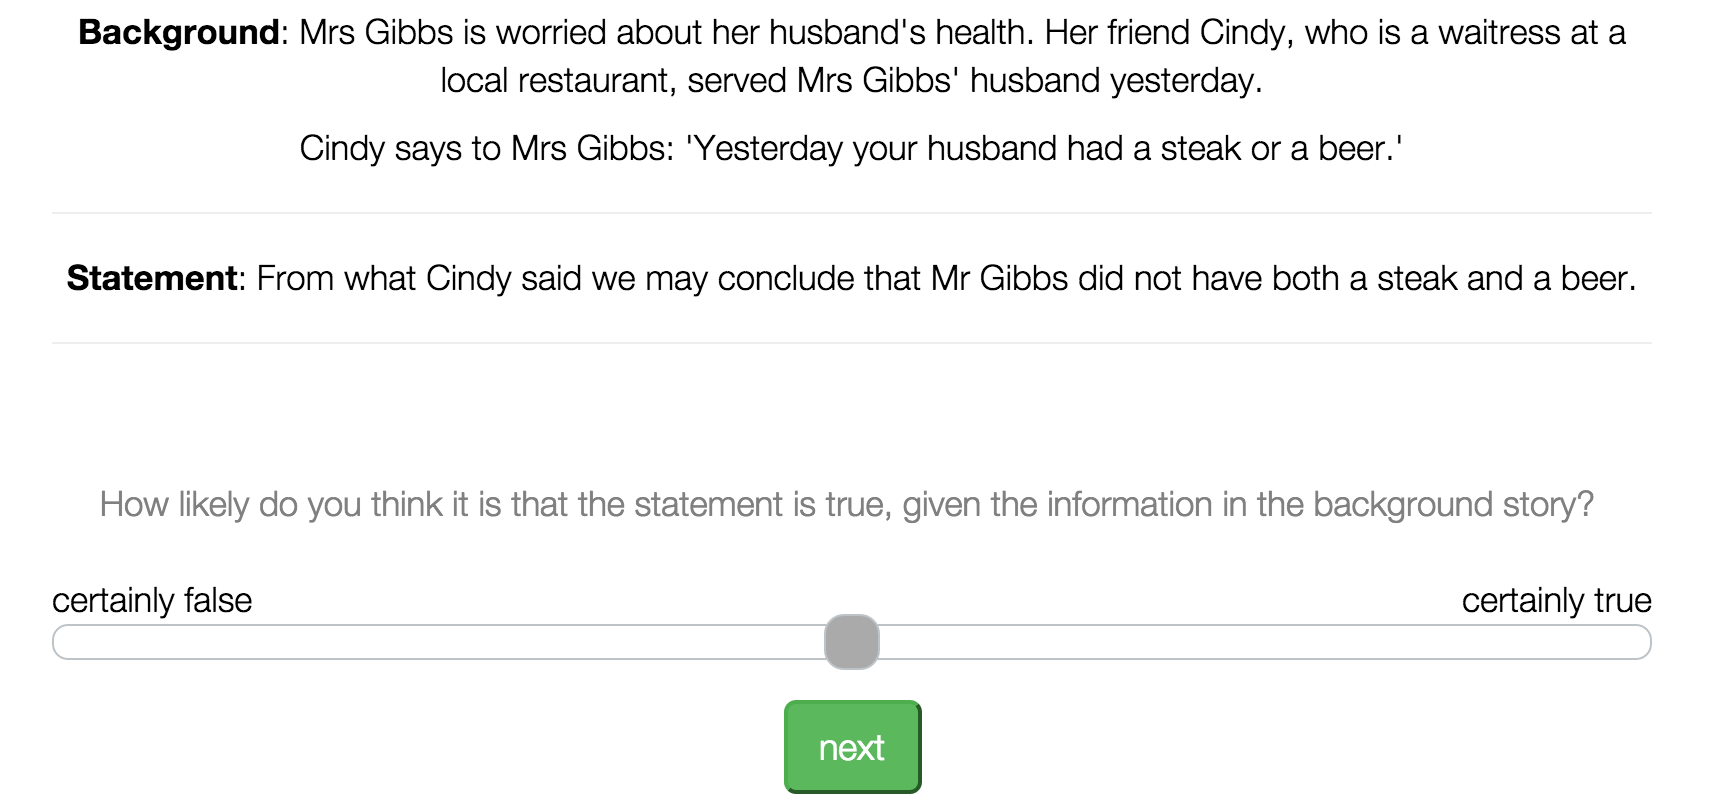
\includegraphics[width = 0.9\textwidth]{pics/expExampleShot.png}
  \caption{Example of a trial \mf{insert pic with example from main text}}
  \label{fig:exampleShot}
\end{figure}

\subsection*{Results}

\paragraph{Data preparation.} We coded the slider-ratings as real numbers ranging from 0
(``certainly false'') to 1 (``certainly true''). Ratings for the two conditional statements in
the prior condition were averaged.

Three participants were excluded from the analysis because they were not self-reported native
speakers of English. We also removed another five participants for obviously deviant answers
(e.g., blindly alternating between maximal agreement and maximal disagreement).\footnote{The
  formal criterion for exclusion was having a \emph{deviance score} greater than a fixed
  threshold, where the deviance score of a participant is the sum of the absolute differences
  between the expected answers for all control questions (0, 0.5, or 1) and the subjects'
  answers. % The mean deviance score was 1.758; its standard deviation is 0.862.
  We set the threshold of exclusion to the mean plus twice the standard deviation. This
  exclusion criterion was also used in all other experiments.}  Consequently, data from a total
of 192 participants made it into our analysis.

Unfortunately, there was a mistake in the formulation of the \emph{Xor}-statement in one of the
vignettes (``Bill's order''). We removed all data from this vignette for our analysis.

\paragraph{Controls.} Control statements were rated as expected, indicating that participants
understood the task in general and paid attention to the background stories. Means, averaged
over all vignettes, for ratings of false (0.26), uncertain (0.48) and true statements (0.81)
are pairwise different (two-population directed $t$-test: $t \approx - 3.72, p < 0.001$ for
false vs.~uncertain; $t \approx - 6.93, p < 0.001$ for uncertain vs.~true).

% Figure~\ref{fig:densityFactors} shows estimated density estimates of the ratings given to the
% four factors of interest, averaged over all vignettes. Competence ratings tend towards full
% uncertainty (mean $\approx 0.51$, standard deviation $\approx 0.34$), similarly for relevance
% ratings (mean $\approx 0.53$, standard deviation $\approx 0.3$). Prior ratings were generally
% lower (mean $\approx 0.37$, standard deviation $\approx 0.25$), and ratings for the disjunctive
% statement higher (mean $\approx 0.63$, standard deviation $\approx 0.33$).

% \begin{figure}[t]
%   \centering

%   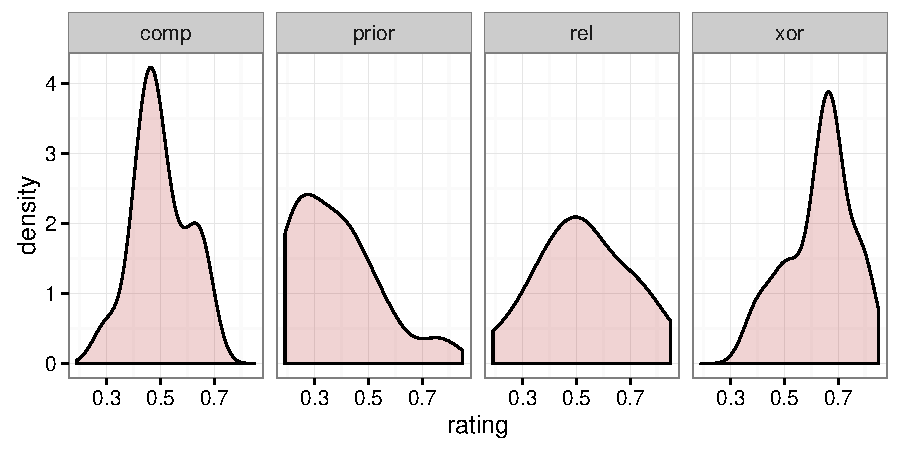
\includegraphics[width = 0.9\textwidth]{pics/densityFactorsExp1.pdf}
  
%   \caption{Density estimates for distribution of ratings across all vignettes}
%   \label{fig:densityFactors}
% \end{figure}

\paragraph{Explanatory factors.} Ratings of relevant explanatory factors are not uniformly
distributed across vignettes, but validate our intuitive pre-classification (see
Figure~\ref{fig:factorBoxPlots}, all high/low contrasts are significant).

\begin{figure}[t]
  \centering

  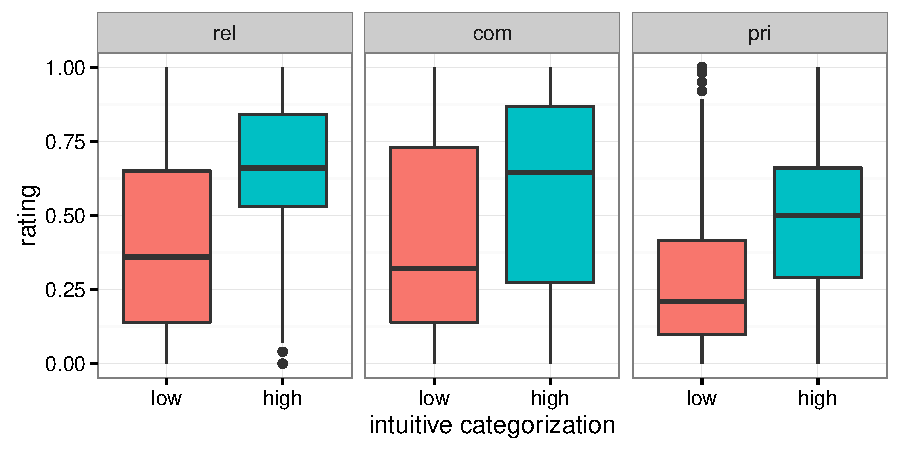
\includegraphics[width = 0.9\textwidth]{pics/factorBoxPlotExp1.pdf}
  
  \caption{Ratings of statements according to intuitive pre-classification in Experiment~1}
  \label{fig:factorBoxPlots}
\end{figure}

Figure~\ref{fig:correlationsExp1} shows the relation of per-vignette mean implicature ratings
and per-vignette mean ratings for the three explanatory factors. From visual inspection, it
seems that relevance and competence are not good predictors of implicature strength, while low prior
plausibility seems to be correlated with high implicature ratings, as expected.

\begin{figure}[t]
  \centering

  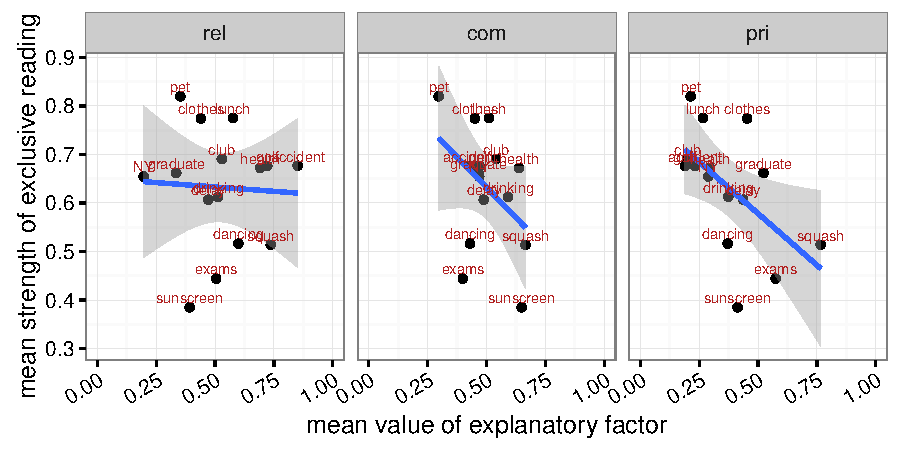
\includegraphics[width = 0.9\textwidth]{pics/correlationExp1.pdf}
  
  \caption{Per-vignette means of ratings of relevance, competence and prior statements
    vs. per-vignette means of implicature rating in Experiment~1}
  \label{fig:correlationsExp1}
\end{figure}

\paragraph{Main analysis.} To check whether factors ``relevance,'' ``prior'' and ``competence''
have an influence on the strength of exclusive readings, we compare regression models of
different complexity. The dependent variable are ratings of the
\emph{Xor}-statement. Explanatory factors \rel, \com, and \pri are, respectively, the means of
the ratings, for each vignette, of the \emph{Relevance}, \emph{Competence} and \emph{Prior}
statements. We take a Bayesian approach to comparing regression models in terms of their Bayes
factors \citep{RouderMorey2012:Default-Bayes-F}, as implemented in the \emph{BayesFactor}
$R$-package. This gives us a more nuanced picture of the relative evidence for models of
different complexity, including information about how much, e.g., the absence of a factor in a
model, is supported by our data.\footnote{All conclusions of theoretical relevance are also
  supported by more traditional, frequentist regression analyses in terms of significance of
  factors and model comparison by AIC.}

\begin{figure}
  \centering
  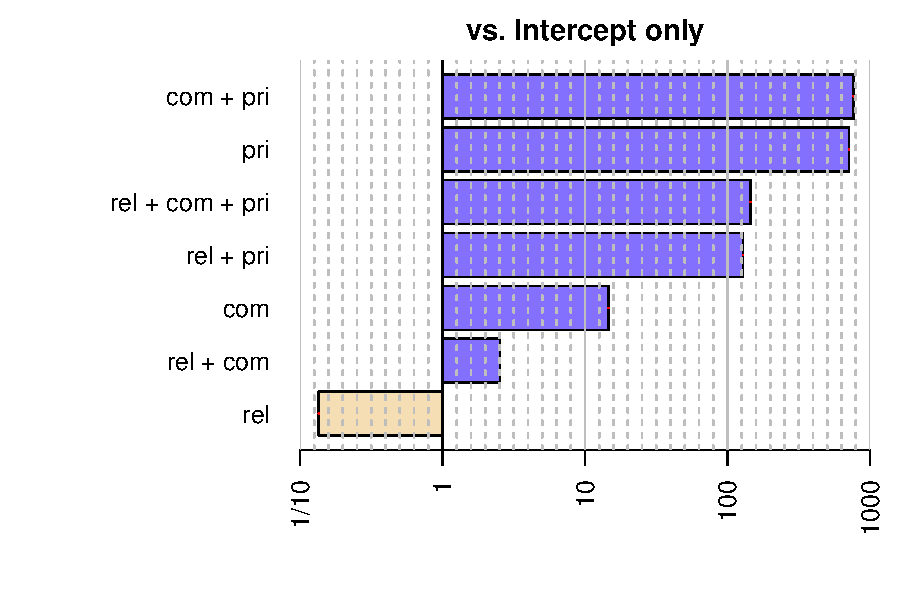
\includegraphics[width = 0.8 \textwidth]{pics/bfsAllExp1.pdf}
  \caption{Bayes factor comparison of different main factor combinations. Notation like ``com +
    pri'' stands for a regression model with main factors \com and \pri.}
  \label{fig:BFs}
\end{figure}


Figure~\ref{fig:BFs} shows the Bayes factors of all regression models that can be built with
our three explanatory variables as main factors. The graph gives the Bayes factor of each
regression model, listed on the right, against the intercept-only model. A model with only \rel
as a main factor, for example, is roughly 8 times worse than the intercept-only model,
suggesting that \rel alone makes no useful contribution to harnessing the variance in
\emph{Xor}-ratings, but only makes for a more complex model. Single main factor \com does make
a significant contribution, compared to the intercept-only model, but a model with single main
factor \pri is more than 30 times more likely, given our data, than the model with just
\com. The best model, by this standard, is a model with \com and \pri as main effects, but
there is no substantial difference between this and the model with only \pri as a main factor.

The main conclusion to be drawn from this analysis is that \rel is a bad, \com an unnecessary,
and \pri the best predictor of strength of exclusive readings.\footnote{This general conclusion
  is also vindicated by more complex analyses that would take interactions and random effects
  for participants into account.} Factor \rel should be omitted for reasons of parsimony (every
model with it is worse than the corresponding one with it), while \com can be omitted at no
substantial loss (adding \com makes models better, but not substantially so, when \pri is
present). Omitting \pri leads to a substantial decline in explanatory power.

Estimates of the posterior distributions over model parameter coefficients for the linear model
that contains all three factors \rel, \com and \pri are shown in
Figure~\ref{fig:densityMCMC}. Noteworthily, most credible values for coefficients for \com are
negative. This is the same for all other models containing factor \com. This means that our
data suggests that the more competent the speaker was felt to be, the lower the strength of the
exclusive reading. This is the reverse of what we would expect from basically all pragmatic
theories. In contrast, the impact of \pri is as expected: the more likely the conjunctive
alternative, the less strong the exclusive reading is felt to be.

\begin{figure}
  \centering
  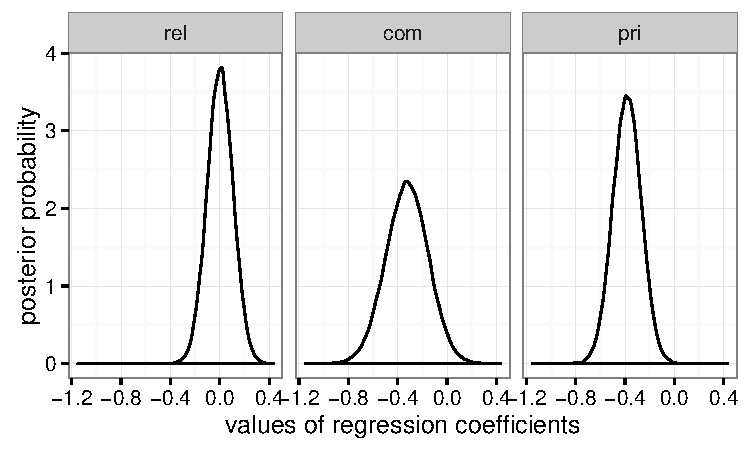
\includegraphics[width=0.8\textwidth]{pics/densityMCMCExp1.pdf}
  \caption{Density estimates of posterior over model parameter coefficients for a linear model
    with all three main factors.}
  \label{fig:densityMCMC}
\end{figure}

\subsection*{Discussion.} Prior plausibility of the conjunctive alternative seems to be the
main explanatory factor of \emph{Xor}-ratings. This is interesting since standard theories
usually do not emphasize the role of prior plausibility. Moreover, it is actually surprising
from the point of view of standard pragmatic theories of exclusive disjunction readings that
relevance does not seem to play an explanatory role and that competence is correlated with
\emph{Xor}-strength in the ``wrong direction,'' so to speak. \mf{more here? or rather later?}

Before drawing firm conclusions, we should address some potential worries about this design and
the evidence that our results provide for or against theoretical positions. First of all, it
could be objected that the way in which we measured factor \pri is inadequate. What matters, so
a possible objection goes, is the prior plausibility of ``$A$ and $B$'' not the mean of the
plausibility of conditionals ``if $A$, $B$'' and ``if $B$, $A$.'' Experiment~2 presents a
follow-up that addresses this issue. Secondly, we should verify that our experimental measures
of relevance, competence and prior do what we would like them to. In order to address this
issue, Experiment~3 looks at scalar quantifier \emph{some} in a parallel design to that of
Experiment~1.


\section{Experiment~2: Prior of conjunctive alternatives}
\label{sec:experiment-2:-prior}

% what is Experiment 2 here is Exp 5 in the data analysis!!!

Experiment~1 formulated target statements which were intended to measure the relative
probability of the conjunctive alternative as a pair of conditional statements ``If disjunct
$A$, then the other disjunct $B$ as well.'' The alternative would be rating of the conjunctive
alternative ``$A$ and $B$.'' We used the former because we reasoned that the latter may have
led to problems in some cases where the overall unconditional probability of $A$ and $B$ being
true together may have been very low. For example, it may be relatively unlikely, among all the
possible choices from a menu, that a character would order both steak and beer. This, despite
the fact that it might be reasonably plausible that, given that a steak (a beer) was ordered, a
beer (a steak) one was ordered as well. Technically, the problem is that for vignettes where we
expected high prior plausibility of the conjunctive alternative, the absolute rating could be
so low that we would not be able to tell it apart from ratings for vignettes where we would
expect a low prior rating. Still, it is prudent to check whether a measure in terms of
conditional statements aligns with a measure in terms of the conjunctive statement. We might be
hard pressed to decide which measure to trust in case of major divergence, but seeing similar
results for both should assure us that we are really measuring what we want to measure.

\subsection*{Design}

Using the same vignettes as in Experiment~1, Experiment~2 asked subjects to rate the
plausibility of conjunctive statements.

\subsection*{Participants}

70 participants were recruited via Amazon's Mechanical Turk, using the same requirements as for
Experiment~1, and paid US\$ 0.50. 

\subsection*{Materials}

All vignettes from Experiment~1 were presented, except for ``Bill's orders,'' the data from
which was not usable due to a coding mistake. Additionally, Experiment~2 introduced a statement
\emph{PriorConj} for each vignette which probed for the (unconditional) probability of the
relevant conjunctive statement (see Appendix~\ref{sec:mater-exper-1}). For the example vignette
used earlier this would be:

\begin{quote}
  \emph{PriorConj} \\ It is likely that Alex bought both a racket and a pair of shoes.
\end{quote}

\subsection*{Procedure}

After reading instructions, which were essentially like in Experiment~1, each subject was
presented with six randomly sampled vignettes. Each vignette was produced without the
``or''-utterance, just like in the prior elicitation conditions for Experiment~1. For each
vignette, subjects first rated a random control statement and then they rated the
\emph{PriorConj} statement.

\subsection*{Results}

We excluded one participant for not identifying as a native speaker of English and another one
for bad performance on the control questions, using the same criterion as for
Experiment~1. Per-vignette means of the given ratings for \emph{Prior}- and
\emph{PriorConj}-statements are highly correlated ($r \approx 0.89, p < 0.0001$, see also
Figure~\ref{fig:correlationPriorMeasures}). We included a factor \textsc{PriCon}, derived from
the means of the conjunctive statements for each vignette, into regression models for
\emph{Xor}-statements, just like in the analysis for Experiment~1. As expected, given their
high degree of correlation, there is no substantial difference between explanatory factors
\textsc{PriCon} and \textsc{Pri}.

\begin{figure}
  \centering
  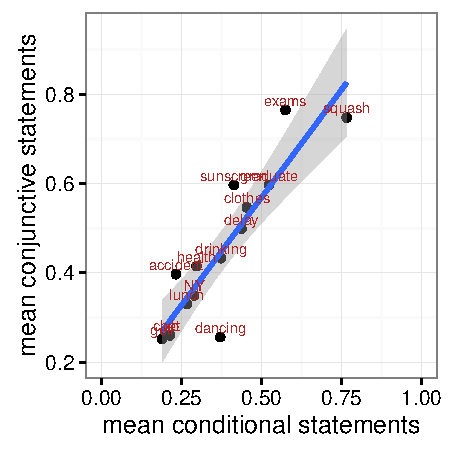
\includegraphics[width=0.5\textwidth]{pics/correlationPriorMeasuresExp1and5.pdf}
  \caption{Correlation of mean prior measures. The $x$-axis has the means (per vignette) of
    mean ratings of conditional \emph{Prior}-statements from Experiment~1. The $y$-axis has the means (per
    vignette) of the ratings of the conjunctive \emph{PriorConj}-statements from Experiment~2.}
  \label{fig:correlationPriorMeasures}
\end{figure}

\subsection*{Discussion}

Against our initial worries, measuring prior expectations in the form of conjunctive statements
seems to deliver basically the same results as a measure based on pairs of conditional
statements. This is reassuring, because it seems to suggest that our measure for prior
expectations is relatively robust and not an artifact of a particular way of
phrasing.\footnote{Interestingly, our initial worry that conditional statements may be more
  natural to rate for plausibility was echoed in a comment which a subject gave after
  completing Experiment~2: ``Most of these statements were pretty nonsensical, I thought it
  would be more straightforward `If A, then B.'''}


\section{Experiment 3}

\subsection*{Design}

It would be tempting to conclude from the results of Experiment~1 that exclusive readings of
disjunctions are not likely the result of a reasoning along the lines of the Gricean recipe
\mf{introduce term ``Gricean recipe''?}. Such a conclusion would be premature, however, as long
as we lack additional evidence that our experimental method is sound and trustworthy. To put
the method to the test, we therefore designed Experiment~3 as a follow-up to
Experiment~1. Experiment~3 has the exact same structure and procedure as Experiment~1, but it
uses material to test for the strength of scalar inferences from \emph{some} to \emph{some but
  not all} and the effect that manipulations of relevance, competence and prior expectations
would have on these.

\subsection*{Participants}

203 participants were drafted on Amazon's Mechanical Turk and paid US\$ 0.80. Payment was not
contingent on responses. Only workers with an IP address from the United States and with a rate
of accepted HITs of at least 90\% were eligible for participation, just as in Experiment~1.

\subsection*{Materials}

Like in Experiment~1, materials consisted of sixteen vignettes, two vignettes per type, where a
type was our intuitive classification of whether the vignette was high or low on dimensions
relevance, competence and prior plausibility (see Appendix~\ref{sec:mater-exper-3} for a full
list). Each vignette came with a background story and an utterance of a sentence with
\emph{some} of some character from the story. For example:

\begin{quote}
  \emph{Background story} \\
  Lucy has to give a talk in front of a big audience of psychologists. She is going to
  criticize one of the dominant theories about schizophrenia. Afterwards, Jacob, who was in the
  audience, chatted with his neighbours.\\[.2cm] 
  \emph{Utterance of \emph{some} sentence}\\
  He tells Lucy: 'Some of the people enjoyed your talk.'
\end{quote}

\noindent As before, each vignette had four target statements to probe into (i) the strength of
the scalar ``not all''-inference, (ii) the relevance of the ``not all''-information for the
listener, (iii) the competence of the speaker and (iv) the prior probability of the proposition
obtained by replacing \emph{some} in the utterance with \emph{all}.\footnote{Statements to
  probe for the prior probability of the \emph{all}-situation were not conditional sentences,
  like in Experiment~1, because we did not expect the unconditional probability of the
  \emph{all}-situation to be rated particularly low in cases where the vignette aimed for a
  high rating and because the unconditional sentences seem fairly natural to rate for
  plausibility.} Here are examples:

\begin{quote}
  \emph{notAll}\\
  From what Jacob said we may conclude that not all of the people enjoyed Lucy's talk.\\[.2cm]
  \emph{Relevance} \\ It is important for Lucy to know whether all of the people enjoyed her talk.\\[.2cm]
  \emph{Competence} \\ Jacob knows whether all of the people enjoyed Lucy's talk. \\[.2cm]
  \emph{Prior} \\ All of the people enjoyed Lucy's talk.
\end{quote}

\noindent As previously, each vignette was also associated with three control statements that
were expected to be certainly true, certainly false, or uncertain. All materials are given in
Appendix~\ref{sec:mater-exper-3}.

\subsection*{Procedure}

The procedure was the same as in Experiment~1, with only slight rewording of the instructions.

\subsection*{Results}

\paragraph{Data preparation.} Four participants were excluded from the analysis because they
were not self-reported native English speakers. Another 6 participants were excluded for poor
performance, by the same criterion as used with Experiment~1. All data from the remaining 193
participants entered into the analysis.

\paragraph{Controls.} Ratings for control statements are unsurprising. Means, averaged over all
vignettes, for ratings of false (0.22), uncertain (0.39) and true statements (0.80) are
pairwise different (two-population directed $t$-test: $t \approx - 3.83, p < 0.001$ for false
vs.~uncertain; $t \approx - 9.98, p < 0.001$ for uncertain vs.~true).

\paragraph{Explanatory factors.} Statements that targeted relevance, competence and prior
probability were rated in accordance with our intuitive classification (see
Figure~\ref{fig:factorBoxPlotsExp3}, all high/low constrasts are significantly different).

\begin{figure}
  \centering

  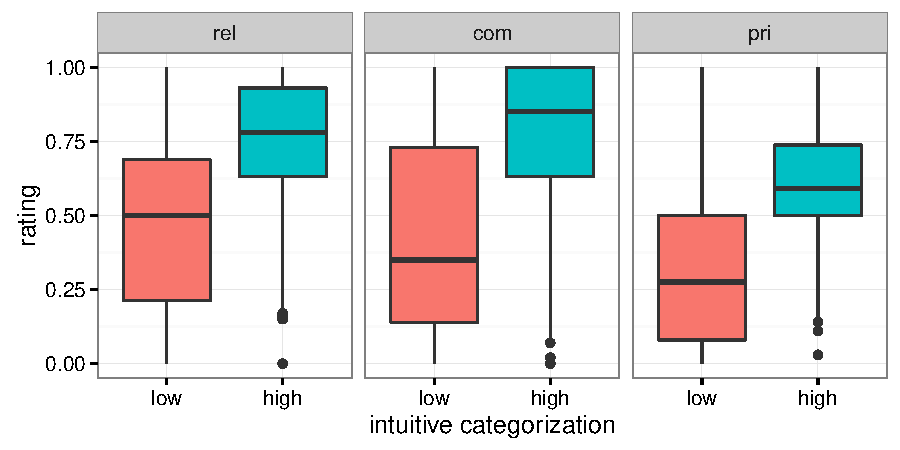
\includegraphics[width = 0.9\textwidth]{pics/factorBoxPlotExp3.pdf}
  
  \caption{Ratings of statements according to intuitive pre-classification in Experiment~3}
  \label{fig:factorBoxPlotsExp3}
\end{figure}

Figure~\ref{fig:correlationsExp3} shows the relation of per-vignette mean implicature ratings
and per-vignette mean ratings for the three explanatory factors. From visual inspection, it
seems that \rel and \com are unlikely good predictors of implicature strength, while low values
of \pri seem to be correlated with high implicature ratings, as expected.

\begin{figure}
  \centering

  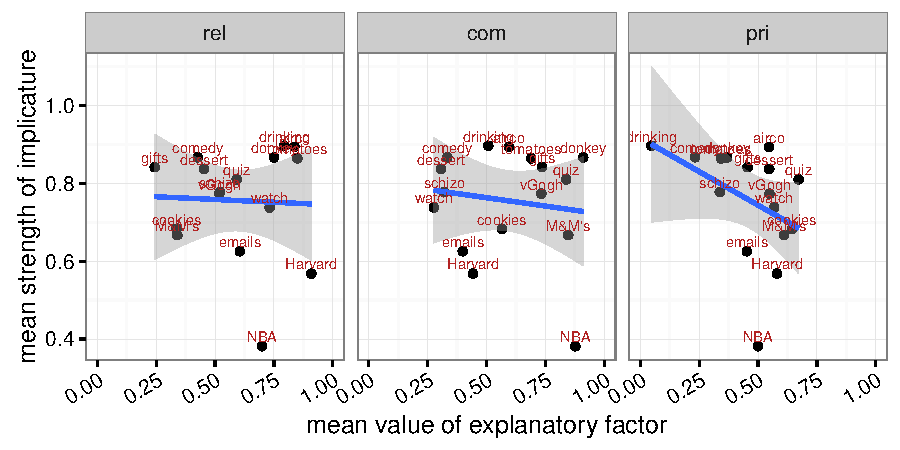
\includegraphics[width = 0.9\textwidth]{pics/correlationExp3.pdf}
  
  \caption{Per-vignette means of ratings of relevance, competence and prior statements
    vs. per-vignette means of implicature rating in Experiment~3}
  \label{fig:correlationsExp3}
\end{figure}

\paragraph{Main analysis.} We want to explain ratings of the \emph{notAll}-statement in terms
of explanatory factors \rel, \pri, and \com, which are, as before, the respective means of
ratings of the corresponding statements for each vignette. Figure~\ref{fig:BFsExp3} gives the
Bayes factors of regression models with our three explanatory variables as main factors. The
best model only contains factor \pri and is made roughly six times more likely by the data than
the two runner-ups which contain additionally \rel or \com. Clearly, the data provides very
strong evidence in favor of all models that include \pri, relative to those which do not.

\begin{figure}
  \centering
  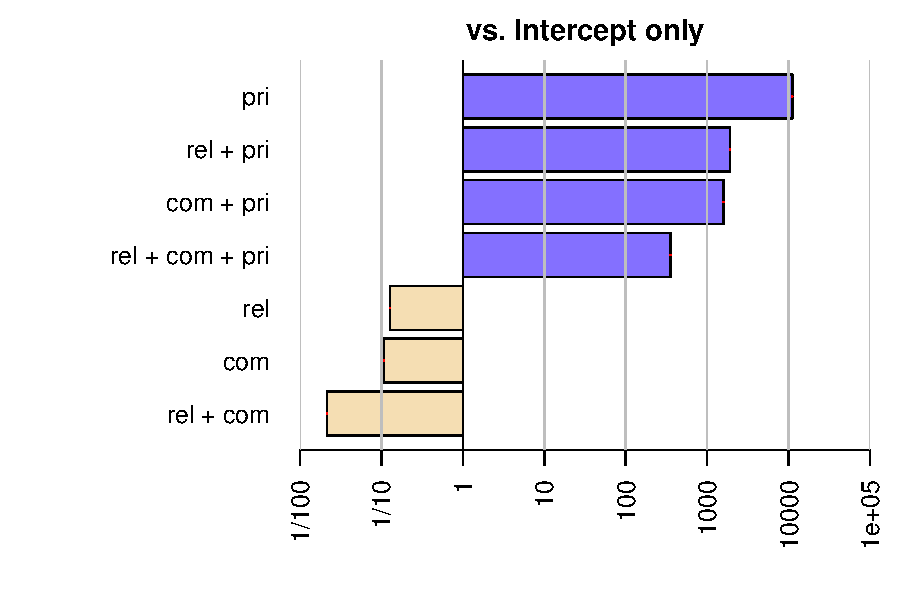
\includegraphics[width = 0.8 \textwidth]{pics/bfsAllExp3.pdf}
  \caption{Bayes factor comparison of different main factor combinations, predicting the
    strength of scalar enrichment of \emph{some} in Experiment~3.}
  \label{fig:BFsExp3}
\end{figure}

\subsection{Discussion}

We could conclude from this analysis that \pri is the key factor in our regression model
comparison for predicting the strength of scalar inferences.\footnote{This is also the case for
  more complex analyses that take interactions and random effects for participants into
  account: the model with only \pri as factor is the best, and every model that contains it is
  strongly favored by the data above any model that does not.} Factors \rel and \com do not
seem to carry extra explanatory power. This would suggest that the behavior of scalar
\emph{some} parallels that of disjunction \emph{or} in terms of which factors seem to influence
the strength of the putative implicatures. 

There is, however, a particular oddity in our data. A look back at
Figure~\ref{fig:correlationsExp3} reveals that one vignette received a surprisingly low mean
score for implicature strength, namely \emph{NBA}. When we compare the ratings of the
\emph{notAll}-statement given for the \emph{NBA} vignette with those given for each other
vignette, we see that all of these fifteen pairwise comparisons shows a significant
difference. No other vignette had that property in Experiment~3, and also no vignette from
Experiment~1 was an ``outlier'' in this sense. Low implicature ratings for this vignette are
particularly surprising, because it was intuitively classified as high relevance, high
competence, and low prior. So, all explanatory factors should, by the standard theory, point
towards high implicature rates. The observed ratings of these factors for this vignette
accorded with intuition. Moreover, the NBA story had remarkably many participants answering
that the likelihood of the implicature was exactly zero. Eight participants provided such a
response; none did so for the next lowest-scoring item. Clearly, this case seems to stand out
in some way.

% One thing that is special about the \emph{NBA} vignette is that not only the speaker is
% introduced as an expert, but also the listener. This vignette is the only one, including
% vignettes from Experiment~1, in which the listener does not seek factual information from the
% speaker. It is the only vignette in which the listener is likely to know whether the
% \emph{all}-situation is true. This may lead subjects to see a different purpose in the
% utterance of the speaker than to provide useful information, if that is measured in terms of
% logical strength. The kind of information that the speaker offers in this vignette is, perhaps,
% much better construed as evidence in favor of a conclusion that is under debate
% \citep{Ducrot1973,AnscombreDucrot1983:Largumentation-,MerinInfoRelSocialDecisionmaking1999,Rooijvan-Rooij2004:Cooperative-ver}. 

% In a sense it is rather unusual that the NBA item should score so low, given how unlikely it is that any one player should score the decisive points in the dying seconds of all playoff games. Indeed, there are several observations indicating that something went wrong with this particular item. First, of course, is the extremely low implicature rating (0.39) compared to the next lowest scoring item (0.58). For comparison, the difference between the second and third lowest scoring items was less than 0.05. Second, the NBA story had remarkably many participants answering that the likelihood of the implicature was 0.00. Eight participants provided such a response; none did so for the next lowest-scoring item.

Here is what we believe went wrong with this item. Consider the \emph{notAll}-statement of this
vignette:

\begin{quote} \emph{notAll} \\
  From what Jason Barley said we may conclude that Greg Jones did not secure victory for his
  team during the last seconds of all of the decisive playoff matches.
\end{quote}

\noindent Rather than directly modifying the noun phrase, the negation modifies the verb phrase
and is separated by three constituents from the noun phrase. This may invite a reading, which
was not intended, in which the negation modifies the verb rather than the noun phrase. In other
words, it invites a reading of the complement of `said' that can be paraphrased as `Greg Jones
failed to secure victory for his team during the last seconds of all of the decisive playoff
matches.' We suspect that participants arrived at this reading because of the amount of
material between the negation and the noun phrase, which invited participants to instead have
the negation modify the verb. Indeed, we found that ratings of exactly zero were overall much
more frequent in cases of VP-negation than in cases of NP-negation. \mf{I don't understand the
  last sentence.  Where did we find that? Should we really mention this? Should we go into the
  NP- vs. VP-negation thing in more detail? Otherwise, maybe drop this?}

In order to test our hypothesis that participants arrived at an unintended reading of the
target statement, we conducted a small follow-up experiment in which we gathered implicature
ratings for a statement that better expressed the intended reading than the one used in
Experiment 3:

\begin{quote} From what Jason Barley said we may conclude that not all of the decisive playoff matches were secured during the last seconds by Greg Jones. \end{quote}

\noindent The follow-up consisted of the NBA story followed by three statements: two control
statements and one target statement. The target statement was varied between the one used in
Experiment 3 (see above) and the alternative one with NP-negation, and was varied between
participants. 40 participants were drafted on Mechanical Turk and were paid \$0.15 for their
participation. They were instructed to, first, read the story carefully and, afterwards,
indicate the likelihood of the corresponding statements on a seven-point Likert scale. We
hypothesised that implicature ratings would be substantially higher for the modified statement
than for the original one.

The normalised implicature ratings for the original statement were slightly lower than in
Experiment 3 (0.25 versus 0.39). Crucially, however, the normalised implicature ratings for the
modified statement were significantly higher and much more in line with what we observed for
the other items (0.76, $t$(29) = 4.28, $p$ $<$ .001). Since the two statements were synonymous
on their intended readings, we consider this compelling evidence that participants in
Experiment 3 arrived at an unintended reading of the target sentence and sufficient reason for
discarding the item from our analysis.

Consequently, we reran the regression model comparison after excluding all data from the
\emph{NBA} vignette. The results are shown in Figure~\ref{fig:BFsExp3noNBA}. The best model
considers only factors \com and \pri. It is more than 6 times likelier, given the data, than
the second best model, which also includes \rel, which in turn is about 3.5 times likelier than
the third model with single factor \pri. Figure~\ref{fig:BFsExp3noNBA_regressionCoefficients}
shows posteriors over regression coefficients for that model with main effects \rel, \com and
\pri. Unlike for the disjunction case in Experiment~1, the effect of factor \com on strength of
scalar enrichment is as expected from standard theory: the more competent a speaker is felt to
be, the stronger the scalar implicature reading.


\begin{figure}
  \centering
  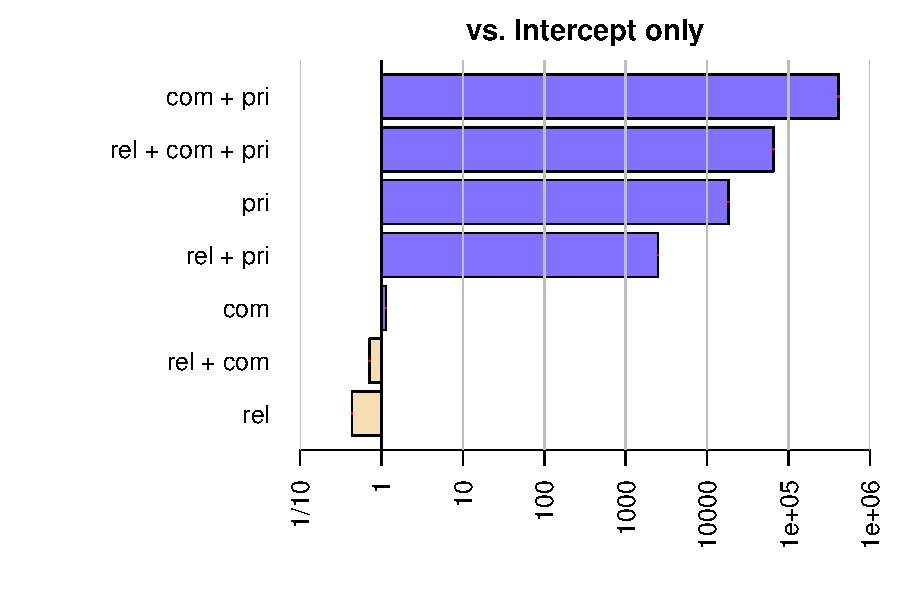
\includegraphics[width = 0.8 \textwidth]{pics/bfsAllExp3_noNBA.pdf}
  \caption{Bayes factor comparison of different main factor combinations, predicting the
    strength of scalar enrichment of \emph{some} in Experiment~3 after excluding data from the
    ``NBA'' scenario.}
  \label{fig:BFsExp3noNBA}
\end{figure}

\begin{figure}
  \centering
  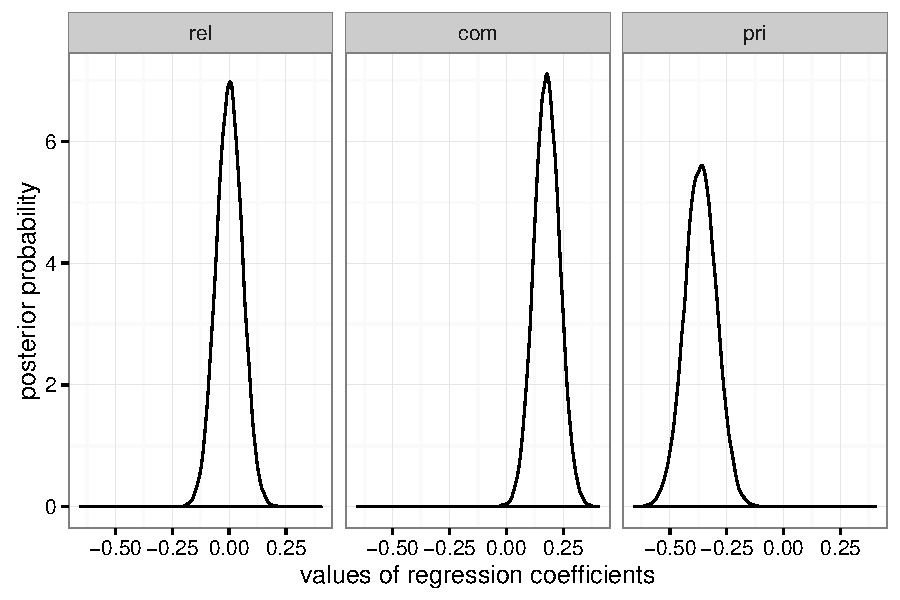
\includegraphics[width = 0.8 \textwidth]{pics/densityMCMCExp3.pdf}
  \caption{\mf{fill me}}
  \label{fig:BFsExp3noNBA_regressionCoefficients}
\end{figure}

In sum, we believe that there are good reasons to exclude the \emph{NBA} vignette from our
analysis, because of an unintended ambiguity in the \emph{notAll}-statement. Doing so, reveals
that factors \pri and \com contribute most to explaining the variance in implicature
strength. Just as for disjunction, relevance seems to be a superflous factor, because any model
without factor \rel is worse than the corresponding one where it is added. This suggests that
the speaker expertise paradox \mf{terminology?} may be a real problem. While manipulations of
competence do have the effects predicted by standard theories of scalar implicature for the
case of \emph{some}, this is not the case for disjunctive readings of \emph{or}. There does
seem to be a difference, which is, as such, already unexpected under standard conceptions.


\section{Experiment~4}

\subsection{Design}

Exclusive readings of disjunctions can also come about by exhaustifying individual disjuncts
(see Section~XYZ). This approach would predict that the strength of an exclusive disjunction
reading of ``$A$ or $B$'' should be positively correlated with the strength of exhaustive
readings that statements of individual disjuncts ``$A$'' and ``$B$'' would receive in the same
context. The purpose of Experiment~4 was therefore to collect data on the strength of
exhaustive readings of such single-disjunct statements in the background contexts used in
Experiment~1. We would then like to investigate whether strengths of exhaustive readings make
for a reliable predictor of strength of exclusive readings across contexts.

\subsection{Participants}

Using the same selection criteria as before, 131 subjects were recruited via Amazon's
Mechanical Turk and paid US\$ 0.50 for participation.

\subsection{Materials}

Experiment~4 used the fifteen vignettes from Experiment~2 (that is excluding the erroneous
``Bill's orders'' scenario). For each vignette we consider the speaker's utterance of single
disjuncts (see Appendix~\ref{sec:mater-exper-1}). Concretely, where Experiment~1 had an
utterance of a disjunction:

\begin{quote}
  \emph{Utterance of disjunction}\\
  Jill says to Danny: `Alex bought a racket or a pair of shoes.'
\end{quote}

\noindent Experiment~2 had two single-disjunct utterances by the same speaker:

\begin{quote}
  \emph{Utterance of disjunct 1}\\
  Jill says to Danny: `Alex bought a racket.' \\[.2cm]
  \emph{Utterance of disjunct 2}\\
  Jill says to Danny: `Alex bought a pair of shoes.'
\end{quote}

\noindent Additionally, each vignette also had corresponding statements that subjects had to
rate:

\begin{quote}
  \emph{Exh1}\\
  From what Alex's girlfriend said we may conclude that Alex did not buy a pair of shoes as well. \\[.2cm]
  \emph{Exh2}\\
  From what Alex's girlfriend said we may conclude that Alex did not buy a racket as well.
\end{quote}

\subsection{Procedure}

The procedure followed that of Experiment~2 very closely. After reading (slightly amended)
instructions and seeing examples for the use of the slider bar, each participant was presented
with six randomly sampled vignettes. Subjects read the background story, followed with an
utterance of disjunct 1 or 2, randomly chosen. Subjects first rated a random control question
and then rated the \emph{Exh1} or \emph{Exh2} statement, depending on which utterance was shown
to them.

\subsection{Results}

Data from one subject was discarded because English was not the self-reported native
language. Another four subjects were removed for bad performance on the control questions,
using the same criterion as before.

\begin{figure}
  \centering
  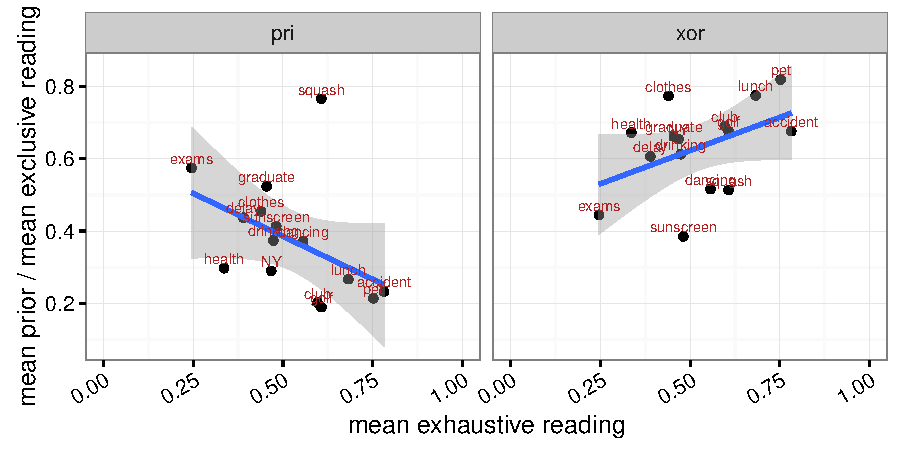
\includegraphics[width=0.9\textwidth]{pics/correlationExhXorPri.pdf}
  \caption{Means of ratings of \emph{Exh}-statements from Experiment~4 ($x$-axis) vs. means of
    ratings of \emph{Prior}-statements and \emph{Xor}-statements from
    Experiment~1 ($y$-axis)}
\label{fig:CorrelationExp1Exp4}
\end{figure}

Figure~\ref{fig:CorrelationExp1Exp4} shows the per-vignette means of the ratings of the
\emph{Exh}-statements plotted against the corresponding mean ratings of the \emph{Prior}- and
\emph{Xor}-statements from Experiment~1. There is no significant correlation between
\emph{Prior}-ratings and \emph{Exh}-ratings ($r \approx -0.44$, $p \approx 0.1$), suggesting
that our measures of prior expectations and exhaustive strength do not coincide. Adding the
per-vignette mean \emph{Exh}-ratings as an additional explanatory factor \exh to the regression
model comparison, we obtain the picture given in Figure~\ref{fig:BayesFactorsExp4}. A model
using single factor \pri to predict \emph{Xor}-ratings is about 8.5 times more likely than a
model using single factor \exh. That means that our data provides evidence for the assumption
that prior expectations are a better explanatory factor of exclusive readings than the strength
of exhaustive readings.

\begin{figure}
  \centering
  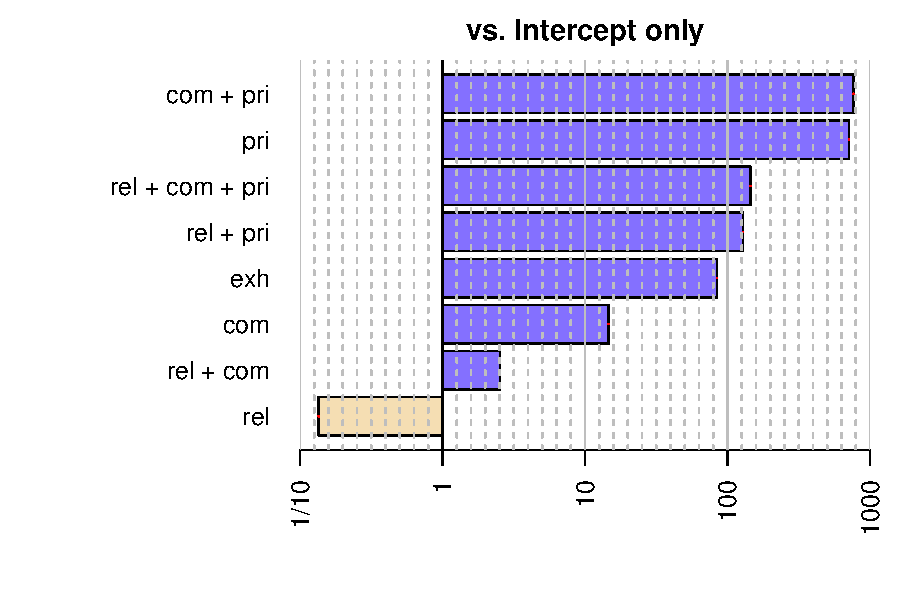
\includegraphics[width=0.9\textwidth]{pics/bfsAllExp4.pdf}
  \caption{Bayes factor comparison of different main factor combinations, predicting the
    strength of exclusive disjunction readings with additional factor \exh from Experiment~4.}
\label{fig:BayesFactorsExp4}
\end{figure}

\subsection{Discussion}

\begin{itemize}
\item something about awareness?
\end{itemize}

\section{General discussion}
\label{sec:general-discussion}

\begin{itemize}
\item there are more factors that influence implicature strength, obviously:
  \begin{itemize}
  \item intonation, speaker-specific adjustments, \dots
  \end{itemize}
\item what about relevance theory?
\end{itemize}

\appendix

\section{Material for Experiments~1, 2 and 4}
\label{sec:mater-exper-1}

\mf{fill me}

\section{Material for Experiment~3}
\label{sec:mater-exper-3}

\mf{fill me}


\bibliography{bibliography}


\end{document}
